\section{Data and choice of offices}\label{app:data}

\paragraph{Lapse records.} PATSTAT's legal-event table (INPADOC) records renewal payments, lapses and expiries for
the offices that report them. I scanned every authority for events in the categories ``cessation'', ``maintenance''
and ``payment'' and measured, for granted invention patents filed 2000--2010: the share with a recorded cessation;
the share of 2000--2005 filings whose first cessation comes within 15 years of filing (lapse rather than expiry);
the number of grants with a domestic first applicant; and the years in which cessations are recorded. Event dates
are effective dates unless missing or set to the placeholder 9999-12-31, in which case publication dates are used.
Table~\ref{tab:coverage} summarises the scan. An office is usable if it records cessation for a large share of grants
continuously over the period.

\begin{table}[ht]
\centering
\begin{threeparttable}
\caption{Lapse records in PATSTAT: candidate emerging-market offices}\label{tab:coverage}
\small
% Source: em-patent-value output/coverage_national.csv (22_coverage_scan.py)
\begin{tabular}{lrccrcl}
\toprule
Office & Grants & Cessation & Lapsed by & Domestic & Years & Verdict \\
 & 2000--10 & recorded & 15 years & grants & recorded & \\
\midrule
Russia         & 301{,}160 & 71\% & 74\% & 128{,}782 & 1987--2022 & included \\
Taiwan         & 306{,}085 & 76\% & 53\% & 124{,}228 & 1994--2025 & included \\
Czech Republic &   7{,}413 & 95\% & 62\% &   3{,}196 & 1990--2025 & included \\
Hungary        &   4{,}160 & 66\% & 43\% &   1{,}290 & 1990--2024 & too few firm patents \\
Poland         &  26{,}623 & 34\% & 35\% &  16{,}171 & 1998--2015 & records stop in 2015 \\
Slovakia, Croatia & 2{,}406 / 2{,}254 & 85 / 97\% & 48 / 67\% & 638 / 1{,}000 & & very small \\
\addlinespace
\multicolumn{7}{l}{\emph{No lapse records ($\leq$1\% of grants):} Mexico, South Africa, India, Argentina, Malaysia,
Ukraine,} \\
\multicolumn{7}{l}{\quad Egypt, Colombia, Saudi Arabia, Romania, Bulgaria, Morocco, Peru} \\
\bottomrule
\end{tabular}
\begin{tablenotes}\footnotesize
\item \emph{Notes:} Granted invention patents filed 2000--2010. Lapsed by 15 years: share of 2000--2005 filings whose
first cessation event comes within 15 years of filing. Domestic grants use the raw first-applicant country and are
understated where it is often missing. China and Korea, in the main sample (Table~\ref{tab:sample}), pass all the tests. Inclusion in the analysis also requires about 1{,}000 domestic firm patents
in the 2000--2005 sample; the Czech Republic (909) is kept as a small Central European case, Brazil (164) and Hungary
(299) are dropped. Ten advanced-economy offices pass the same tests; the five largest by domestic firm patents with
full records are used.
\end{tablenotes}
\end{threeparttable}
\end{table}

\paragraph{Advanced-economy offices.} Ten advanced-economy offices have usable records (the United States, Japan,
Germany, the United Kingdom, France, Canada, Australia, Spain, the Netherlands and Sweden). To match the five
emerging-market offices I use the five with the most domestic firm patents.

\begin{figure}[ht]
\centering
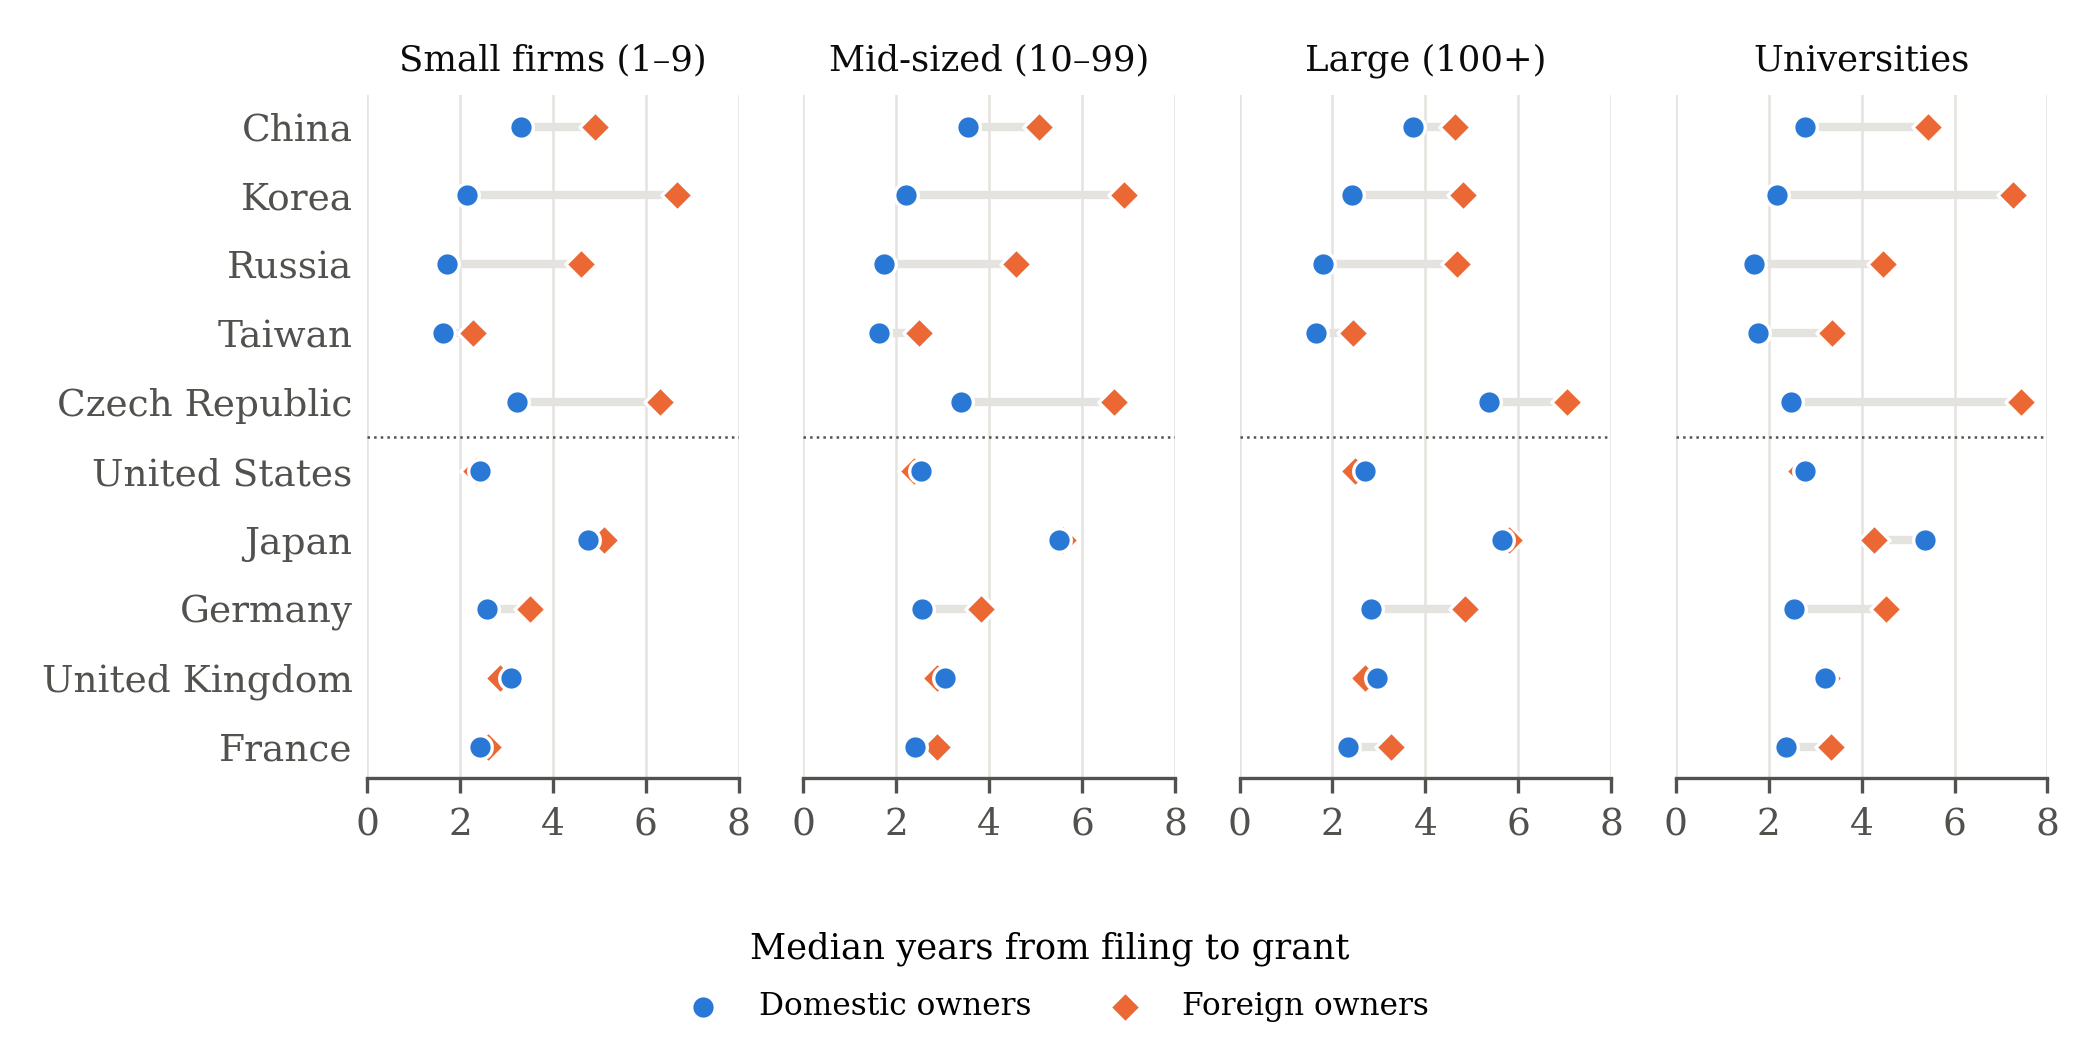
\includegraphics[width=\textwidth]{figures/fig1_grant_lags.png}
\caption{Grant lags by owner and firm size}\label{fig:lags}
\figurenotes{Median years from filing to the first grant publication, patents of Table~\ref{tab:sample}; firm size
as in Table~\ref{tab:sample}. Circles: domestic owners; diamonds: foreign owners. No Czech firm has 100 or more
inventions. Many foreign applications enter through the international (PCT) route, which adds up to 30 months before
national examination begins. Source: em-patent-value output/sample\_lags.csv.}
\end{figure}

\paragraph{Owners and quality.} Owner identities are PATSTAT's harmonised applicant names (HAN). Sector comes from
PATSTAT's sector allocation. Applications with no recorded applicant have no HAN or sector and drop out of the
owner-group estimates; they are common among domestic patents in Russia and foreign patents in Japan and Korea, where
national records often omit applicants.

\paragraph{Corporate groups.} Firm size is the number of distinct DOCDB families filed worldwide in 2000--2005 by the
owner's corporate group. Multinationals and Chinese groups file under several HANs (local subsidiaries, name variants),
so the HAN alone classes units of large groups as small or mid-sized. Company HANs are linked when they share a core
name in the same country (legal forms, bracketed text and trailing place names removed), when a HAN's core name starts
with the first two distinctive words of a group with 100 or more families, or when at least half of a HAN's families
(and at least two) are shared with such a group. Dictionary words, place names and generic business words in several
languages never count as distinctive, and person names are never linked. In audits of randomly drawn reclassified
owners, these links were correct in about 95\% of cases. A group's size is the largest of the owner's own families,
its group total and the totals of linked large groups. The change matters most for foreign owners: in China, 44\% of
foreign small-firm patents move to a larger class against 6\% of domestic ones. A wider definition that also links
owners by brand words anywhere in the name (Sony, Haier, Sinopec units) catches more groups but also unrelated firms
that share a surname or a place name; it is used as a robustness check.

Citation counts are citing DOCDB families. Blocking citations are citing applications
whose search report marks the patent X or Y. Grant lag is measured to the first publication flagged as a grant.

\section{Survival: additional results}\label{app:results}

Table~\ref{tab:bycountry} compares each emerging-market office with the advanced-economy offices,
Table~\ref{tab:rich} collects the robustness checks of Section~\ref{sec:survival}, and Table~\ref{tab:within} shows the
domestic--foreign gap within each office, the benchmark that the other tables difference against. All use the
preferred specification of Table~\ref{tab:survival} and firm size by corporate group.


\begin{table}[ht]
\centering
\begin{threeparttable}
\caption{Extra domestic--foreign survival gap, each emerging-market office against the advanced-economy offices (pp)}\label{tab:bycountry}
\small
% Generated by em-patent-value code/38_paper_exhibits.py (main_by_office.csv); do not edit by hand
\begin{tabular}{lccccc}
\toprule
 & All owners & Small firms & Mid-sized firms & Large firms & Universities \\
 & & (1--9) & (10--99) & (100+) & \\
\midrule
China          & $-0.8$ & $0.7$ & $7.8^{***}$ & $5.1$ & $-19.7^{***}$ \\
               & (2.4) & (0.8) & (1.7) & (4.2) & (2.8) \\
Korea          & $4.8^{**}$ & $3.9^{**}$ & $11.8^{***}$ & $5.8^{**}$ & $2.8$ \\
               & (2.0) & (1.7) & (1.8) & (2.7) & (5.8) \\
Russia         & $-17.2^{***}$ & $-7.9^{***}$ & $-25.0^{***}$ & $-12.8$ & $-10.0^{*}$ \\
               & (1.4) & (2.2) & (6.4) & (8.3) & (5.2) \\
Taiwan         & $9.6^{***}$ & $-0.3$ & $4.3^{**}$ & $10.8^{**}$ & $27.8^{***}$ \\
               & (3.6) & (1.6) & (2.1) & (4.8) & (4.6) \\
Czech Rep.     & $-7.1^{**}$ & $-1.0$ & $-11.6^{**}$ & -- & -- \\
               & (3.2) & (5.3) & (4.8) &  &  \\
\bottomrule
\end{tabular}
\begin{tablenotes}\footnotesize
\item \emph{Notes:} Each row is \PaperRef{Table~2}{Table~\ref{tab:survival}} (columns 2--6, preferred specification) re-estimated on one emerging-market office and the five advanced-economy offices: the extra domestic--foreign gap in survival eight years after grant in that office relative to the advanced-economy offices. Standard errors clustered by owner in parentheses. --: fewer than 100 domestic or foreign patents. $^{*}$~$p<0.1$, $^{**}$~$p<0.05$, $^{***}$~$p<0.01$.
\end{tablenotes}
\end{threeparttable}
\end{table}


\begin{table}[ht]
\centering
\begin{threeparttable}
\caption{Robustness of the extra domestic gap in emerging-market offices (pp)}\label{tab:rich}
\small
% Generated by em-patent-value code/38_paper_exhibits.py (main_robust.csv, step 37); do not edit by hand
\begin{tabular}{lccccc}
\toprule
 & All owners & Small firms & Mid-sized & Large firms & Universities \\
\midrule
Preferred specification (Table 2) & $4.9^{***}$ & $0.3$ & $6.9^{***}$ & $6.7^{***}$ & $-6.2^{*}$ \\
 & (1.8) & (0.7) & (1.1) & (2.4) & (3.7) \\
\quad s.e., clustered by office & [2.2] & [1.8] & [2.5] & [2.0] & [10.3] \\
\quad $p$, wild cluster bootstrap & 0.13 & 0.88 & 0.09 & 0.08 & 0.64 \\
\quad $p$, randomization inference & 0.47 & 0.85 & 0.30 & 0.34 & 0.65 \\
\addlinespace
Linear citation slopes & $5.5^{***}$ & $0.3$ & $7.3^{***}$ & $7.4^{***}$ & $-6.4^{*}$ \\
 & (1.8) & (0.6) & (1.1) & (2.5) & (3.6) \\
No grant-lag controls & $6.1^{***}$ & $2.8^{***}$ & $8.4^{***}$ & $7.7^{***}$ & $-5.5$ \\
 & (1.6) & (0.6) & (1.0) & (2.4) & (3.6) \\
\addlinespace
Alive 12 years after filing & $3.3^{*}$ & $-1.1$ & $4.4^{***}$ & $4.9^{*}$ & $-5.5$ \\
 & (2.0) & (0.7) & (1.2) & (2.7) & (4.2) \\
Reweighted to domestic citations & $2.9$ & $0.3$ & $6.9^{***}$ & $3.4$ & $-8.2^{**}$ \\
 & (1.8) & (0.9) & (1.4) & (2.6) & (3.5) \\
Same-office citations & $-3.6^{*}$ & $-6.0^{***}$ & $0.4$ & $-3.1$ & $-14.6^{***}$ \\
 & (1.9) & (0.6) & (1.1) & (2.5) & (3.7) \\
Identical fees & $4.7^{***}$ & $0.0$ & $4.6^{***}$ & $6.5^{***}$ & $-7.1^{*}$ \\
 & (1.8) & (0.7) & (1.2) & (2.5) & (3.8) \\
\addlinespace
Foreign groups' affiliates dropped & $4.8^{***}$ & $0.3$ & $7.0^{***}$ & $6.6^{***}$ & $-6.2^{*}$ \\
 & (1.8) & (0.7) & (1.1) & (2.5) & (3.7) \\
Applicant-record country only & $7.0^{***}$ & $1.1$ & $8.2^{***}$ & $9.2^{***}$ & $-2.7$ \\
 & (2.1) & (0.7) & (1.2) & (2.9) & (3.9) \\
\addlinespace
Bound for unobservables (Oster) & $18.7$ & $7.7$ & $17.9$ & $16.2$ & $19.5$ \\
\bottomrule
\end{tabular}
\begin{tablenotes}\footnotesize
\item \emph{Notes:} $\delta$ of \PaperRef{Table~2}{Table~\ref{tab:survival}}, all ten offices; each row changes one thing in the preferred specification. Inference across offices, for the preferred specification: standard errors clustered by office in brackets; $p$-values from a wild cluster bootstrap by office (Webb weights, null imposed) and from randomization inference over the 252 assignments of five of the ten offices to the emerging-market group. Linear citation slopes: in place of citation bins. Alive 12 years after filing: outcome counted from filing, with the grant-lag controls. Reweighted: foreign patents weighted to the domestic citation-bin distribution of their office. Same-office citations: citations from applications filed at the same office, a narrower and noisier measure, in place of family citations. Identical fees: without Russia (separate non-resident fees until 2012), patents alive three years after grant (early-year discounts for domestic owners in China and Korea), Chinese grants to 2010 and Korean grants to 2006, so that domestic and foreign owners pay the same fees in every year the outcome covers. Foreign groups' affiliates dropped: domestic patents of applicants linked to a large group from another country removed. Applicant-record country: drops owners whose country is imputed. Oster bound: coefficient if unobservables moved it as much, relative to their explanatory power, as the controls do ($\beta = 1$, $R_{\max} = 1.3 R^2$). Standard errors clustered by owner in parentheses. $^{*}$~$p<0.1$, $^{**}$~$p<0.05$, $^{***}$~$p<0.01$.
\end{tablenotes}
\end{threeparttable}
\end{table}


\begin{table}[ht]
\centering
\begin{threeparttable}
\caption{Domestic minus foreign owners within each office, not relative to the advanced economies (pp)}\label{tab:within}
\small
% Generated by em-patent-value code/38_paper_exhibits.py (main_within_office.csv); do not edit by hand
\begin{tabular}{lccccc}
\toprule
 & All owners & Small firms & Mid-sized firms & Large firms & Universities \\
 & & (1--9) & (10--99) & (100+) & \\
\midrule
\multicolumn{6}{l}{\emph{A. Emerging-market offices}} \\
China          & $7.4^{***}$ & $4.9^{***}$ & $14.4^{***}$ & $10.5^{***}$ & $-15.4^{***}$ \\
               & (2.4) & (0.7) & (1.6) & (3.9) & (2.4) \\
Korea          & $10.8^{***}$ & $7.3^{***}$ & $16.9^{***}$ & $10.8^{***}$ & $7.2$ \\
               & (2.1) & (1.7) & (1.8) & (2.4) & (5.4) \\
Russia         & $-19.1^{***}$ & $-14.5^{***}$ & $-32.2^{***}$ & $-19.0$ & $-10.1^{**}$ \\
               & (2.9) & (2.9) & (7.9) & (13.0) & (4.9) \\
Czech Rep.     & $0.7$ & $5.9$ & $-1.4$ & -- & -- \\
               & (3.5) & (6.0) & (5.3) &  &  \\
Brazil         & $2.4$ & $-1.4$ & $-5.7$ & $44.8^{***}$ & $11.4$ \\
               & (6.3) & (13.1) & (11.3) & (13.6) & (31.4) \\
\addlinespace
\multicolumn{6}{l}{\emph{B. Advanced-economy offices}} \\
United States  & $3.8^{***}$ & $2.2^{***}$ & $3.8^{***}$ & $3.8^{*}$ & $4.5^{**}$ \\
               & (1.4) & (0.4) & (0.5) & (2.0) & (2.0) \\
Japan          & $17.7^{***}$ & $18.6^{***}$ & $21.4^{***}$ & $16.4^{***}$ & $34.0^{***}$ \\
               & (1.8) & (1.6) & (1.5) & (2.1) & (6.9) \\
Germany        & $2.6$ & $7.3^{***}$ & $-1.9$ & $2.6$ & $1.4$ \\
               & (1.8) & (1.6) & (2.1) & (2.4) & (10.2) \\
United Kingdom & $1.6$ & $1.2$ & $3.6$ & $1.1$ & $-15.2^{***}$ \\
               & (2.1) & (2.1) & (2.6) & (4.8) & (4.4) \\
France         & $-1.1$ & $1.1$ & $0.4$ & $-1.4$ & $-2.6$ \\
               & (2.9) & (2.1) & (2.5) & (3.9) & (6.6) \\
\bottomrule
\end{tabular}
\begin{tablenotes}\footnotesize
\item \emph{Notes:} Coefficient on domestic owner from a separate regression for each office and owner group: the domestic--foreign gap in survival eight years after grant within that office, at the mean grant lag, with filing-year, field, citation-bin and grant-lag-year effects, a domestic $\times$ grant-lag slope (and owner-group effects for all owners). Unlike \PaperRef{Table~2}{Table~\ref{tab:survival}} and Table~\ref{tab:bycountry}, these gaps are not differenced against the advanced-economy offices; panel B shows the benchmark those tables difference against. Standard errors clustered by owner in parentheses. --: fewer than 100 domestic or foreign patents. $^{*}$~$p<0.1$, $^{**}$~$p<0.05$, $^{***}$~$p<0.01$.
\end{tablenotes}
\end{threeparttable}
\end{table}




\section{Owner constraints: additional results}\label{app:constraints}

Table~\ref{tab:sales} reports the sale test of Section~\ref{sec:constraints} by office and type of transfer, and the emerging-minus-advanced
difference under three definitions: all recorded transfers in the six offices that record them, sales to unrelated
buyers in the three offices whose records name the owners, and the latter counted from grant, the definition used to
calibrate the markets-for-technology lever.

\begin{table}[ht]
\centering
\begin{threeparttable}
\caption{Survival five years after a sale: arm's-length and related transfers (pp)}\label{tab:sales}
\small
% Generated by em-patent-value code/38_paper_exhibits.py (sales_arms_*.csv, step 34b); do not edit by hand
\begin{tabular}{lcccc}
\toprule
 & Small firms & Mid-sized & Large firms & Universities \\
\midrule
\multicolumn{5}{l}{\emph{A. Premium by office and type of transfer}} \\
China, all transfers & $12.0^{***}$ & $7.2^{***}$ & $-1.0$ & $44.7^{***}$ \\
 & (0.8) & (1.9) & (3.9) & (2.1) \\
China, arm's-length & $11.4^{***}$ & $4.7^{*}$ & $-6.6^{*}$ & $44.9^{***}$ \\
 & (0.9) & (2.5) & (3.9) & (2.2) \\
China, related & $12.8^{***}$ & $11.0^{***}$ & $7.2^{*}$ & $46.5^{***}$ \\
 & (1.3) & (2.7) & (4.2) & (3.2) \\
Germany, all transfers & $5.8^{**}$ & $4.7^{*}$ & $2.3$ & $-1.6$ \\
 & (2.4) & (2.7) & (3.8) & (6.7) \\
Germany, arm's-length & $0.6$ & $0.4$ & $9.5^{**}$ & $-2.0$ \\
 & (4.0) & (5.0) & (4.5) & (8.9) \\
Germany, related & $9.2^{***}$ & $7.0^{**}$ & $-0.7$ & $-1.2$ \\
 & (3.0) & (3.1) & (5.3) & (7.4) \\
France, all transfers & $5.4^{**}$ & $6.0^{**}$ & $7.3$ & $3.3$ \\
 & (2.1) & (2.9) & (6.3) & (3.5) \\
France, arm's-length & $9.2$ & $16.7^{***}$ & $4.3$ & -- \\
 & (5.9) & (5.5) & (10.0) &  \\
France, related & -- & -- & $-2.1$ & -- \\
 &  &  & (7.2) &  \\
\addlinespace
\multicolumn{5}{l}{\emph{B. Emerging minus advanced}} \\
All transfers, six offices & $7.0^{***}$ & $7.4^{***}$ & $-3.5$ & $44.0^{***}$ \\
 & (1.1) & (2.0) & (4.0) & (4.3) \\
Arm's-length, China vs.\ Germany, France & $8.0^{**}$ & $0.4$ & $-15.3^{***}$ & $43.1^{***}$ \\
 & (3.5) & (4.7) & (5.8) & (8.7) \\
Arm's-length, counted from grant & $3.8$ & $4.8$ & $-2.4$ & $38.4^{***}$ \\
 & (3.4) & (5.0) & (13.4) & (7.9) \\
\bottomrule
\end{tabular}
\begin{tablenotes}\footnotesize
\item \emph{Notes:} Panel B, six offices: China and Russia against Japan, Germany, the United Kingdom and France, the offices that record sales of granted patents. Domestic owners' patents alive and not yet sold 4--8 years after filing (last row: 1--5 years after grant); survival five years later of patents sold in the next year minus that of unsold patents; log citations up to the landmark and the grant lag as controls; standard errors clustered by owner. Transfers are classified from the former and new owners' names, which only the Chinese (to 2015), German and French records carry (French records name only the new owner; the former owner is then the patent's applicant): related transfers share a name or a distinctive name word (renames, restructurings, moves within a group), arm's-length transfers do not; partial transfers (France) and transfers without names are left out of the arm's-length rows. Firm size by corporate group. --: fewer than 30 sales. $^{*}$~$p<0.1$, $^{**}$~$p<0.05$, $^{***}$~$p<0.01$.
\end{tablenotes}
\end{threeparttable}
\end{table}



\begin{figure}[ht]
\centering
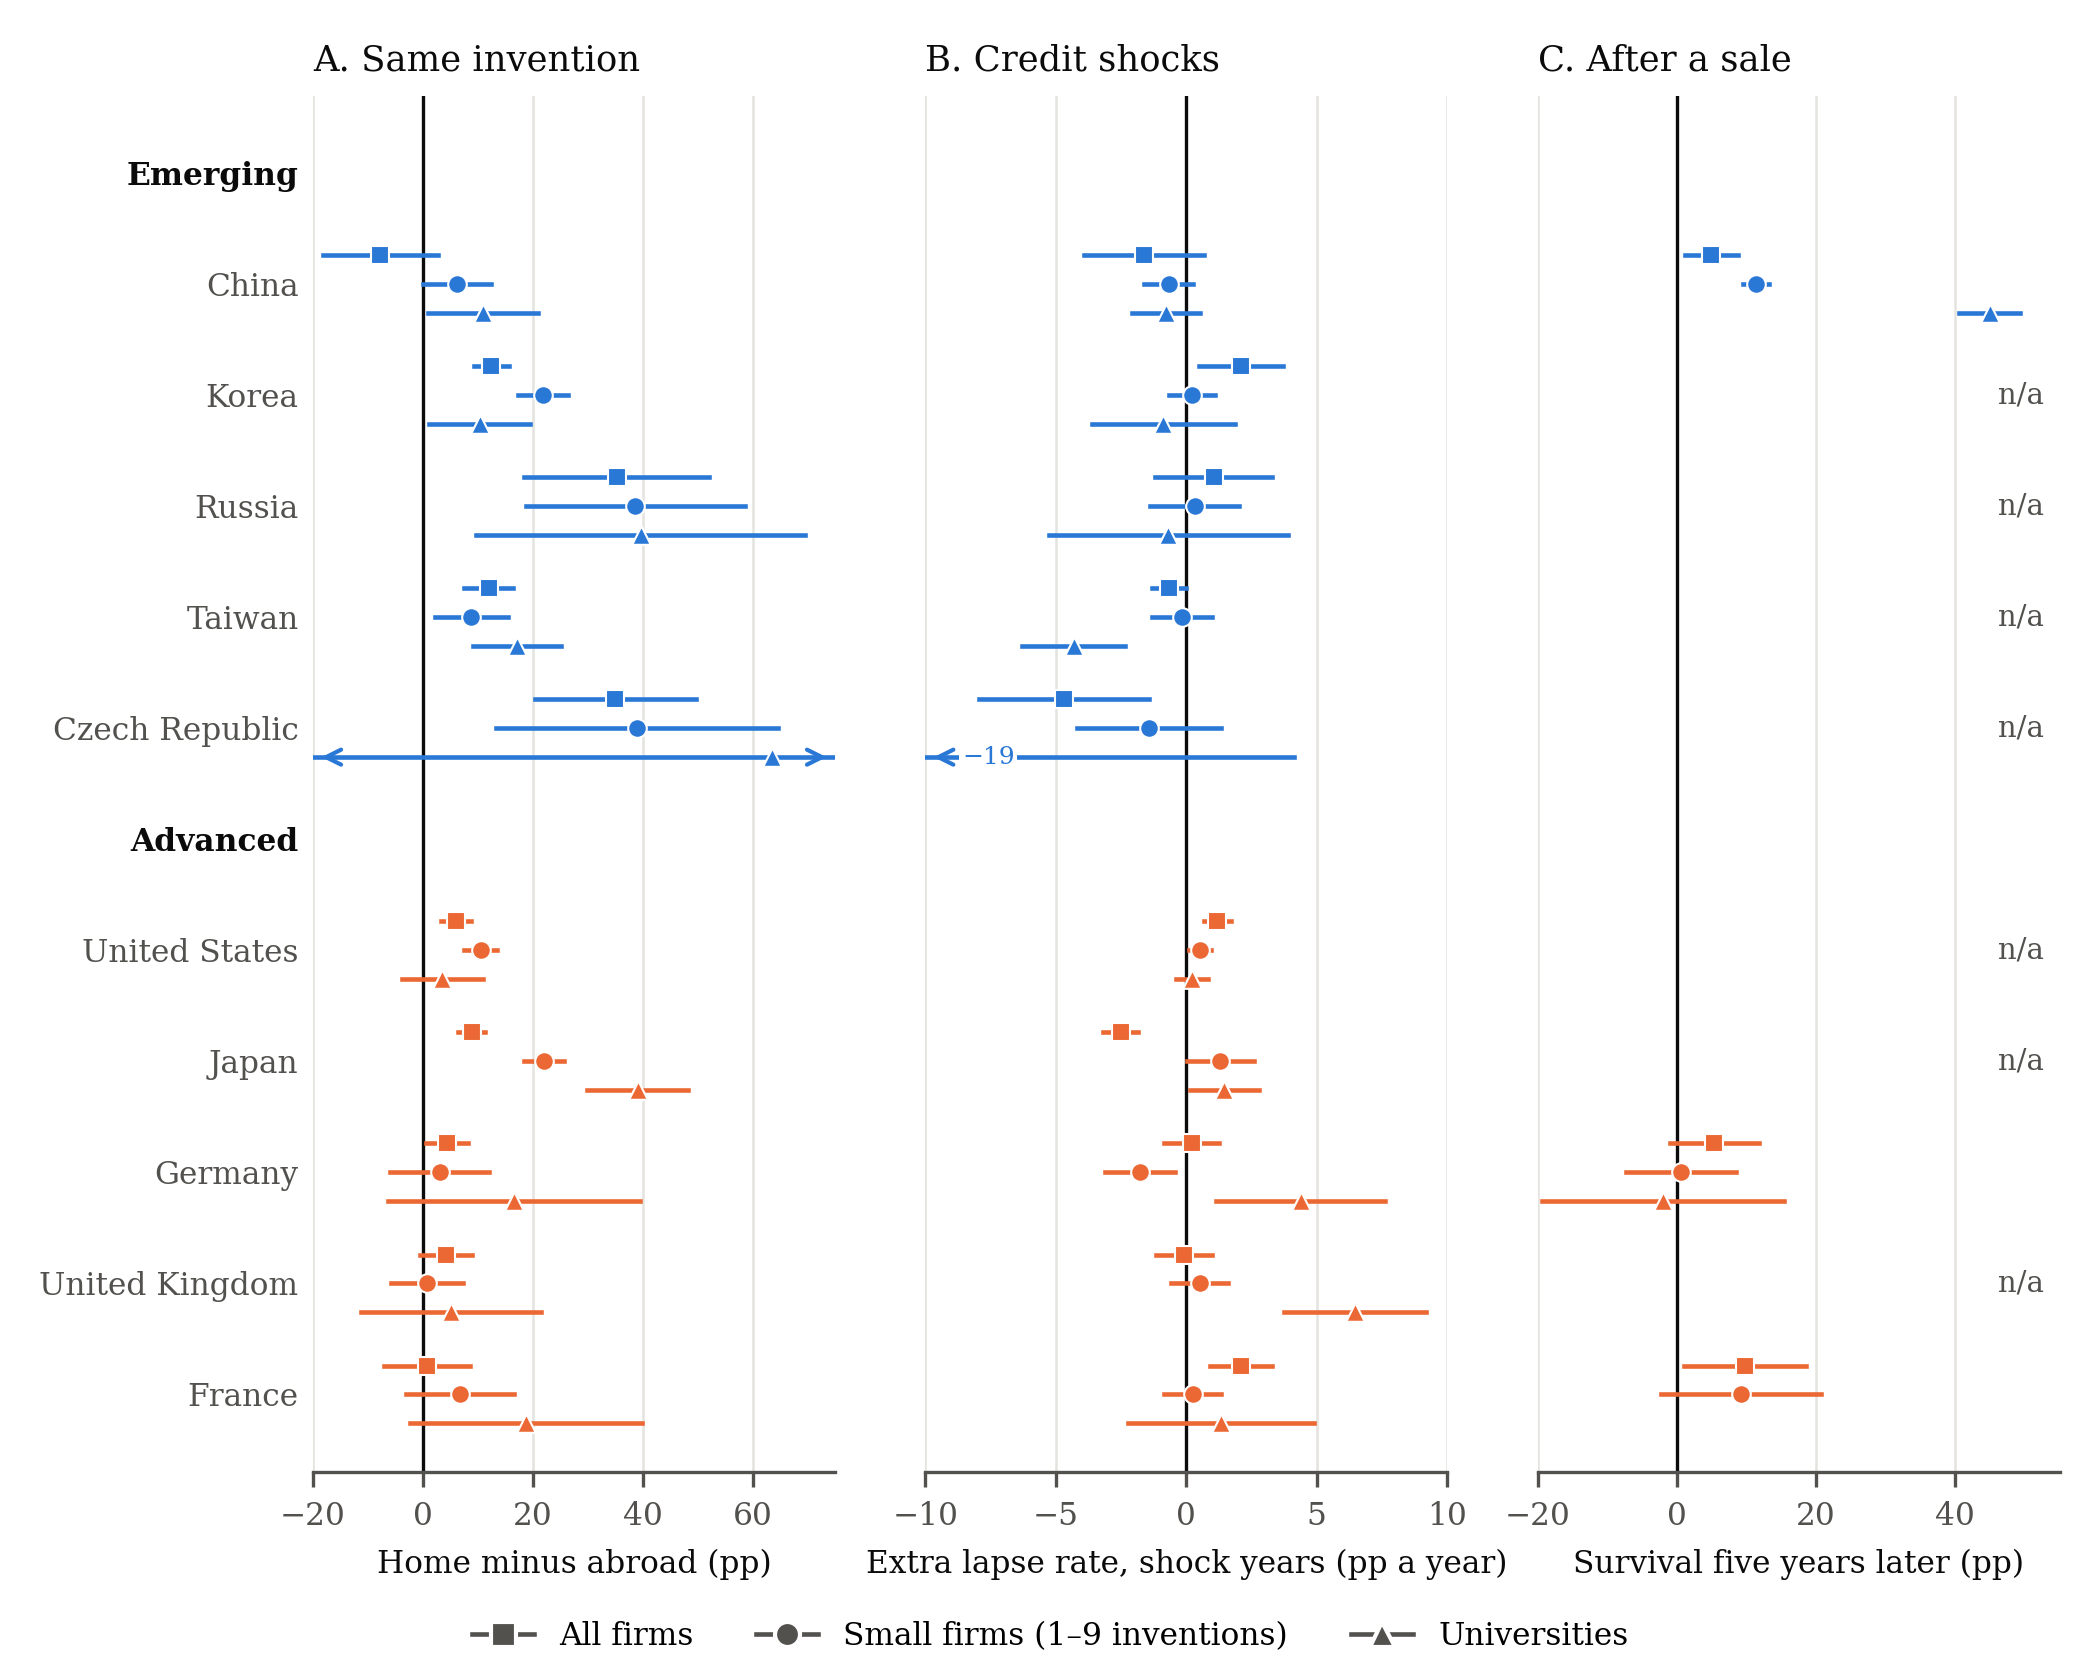
\includegraphics[width=\textwidth]{figures/fig6_constraints_country.png}
\caption{Owner-constraint tests by country}\label{fig:constraints-country}
\figurenotes{Point estimates with 95\% confidence intervals, in percentage points; blue: emerging economies, orange: advanced economies; squares: all firms, circles: small firms (1--9 inventions filed worldwide in 2000--2005), triangles: universities. Arrows: interval beyond the axis; a number replaces a point beyond it. The estimates of Figure~\ref{fig:constraints} by country of origin (A) or office (B, C), specified as in footnote~\ref{fn:specs}. n/a: no sales of granted patents recorded (Korea records changes of owner only before grant).}
\end{figure}

\begin{table}[ht]
\centering
\begin{threeparttable}
\caption{Responses of small firms to fee changes}\label{tab:fees}
\small
% Source: em-patent-value output/fee_response.csv (17_fee_response.py; size 2000-2005)
\begin{tabular}{@{}l>{\raggedright\arraybackslash}p{0.42\textwidth}cc@{}}
\toprule
Office & Variation & Coefficient & Elasticity \\
\midrule
China & 70\% off fee-years 1--3; 85\% off years 1--6 (2016) and 1--10 (2018), intent to treat & 0.0008 (0.0005) & 0.02 \\
Korea & 30\% off years 4--6 (2014) and 4--9 (2016), 50\% off years 4+ (2018) & $-0.033$ (0.027) & n.i. \\
United States & stage-specific fee changes (2004, 2013, 2020) & 0.047 (0.019) & 0.26 \\
\quad placebo: 100+ firms & stage-specific fee changes & 0.009 (0.048) & 0.05 \\
United States & 2022 small-entity discount (50\% to 60\%) & 0.023 (0.024) & -- \\
France & SME reductions for years 2--7 (2005, 2008), intent to treat & $-0.083$ (0.027) & n.i. \\
\bottomrule
\end{tabular}
\begin{tablenotes}\footnotesize
\item \emph{Notes:} n.i.: not identified. Panel of renewal decisions of small firms (1--9 inventions filed worldwide in 2000--2005); outcome:
the patent lapses at that payment. Regressor: log of the fee or fee multiplier the owner faces; controls are firms with
100 or more inventions, which are not eligible. Korean lapse records end in 2019, so only the 2014--2018 windows identify the Korean discounts. The French
estimate has the wrong sign and keeps it with small-firm $\times$ filing-cohort effects ($-0.100$, 0.033); it is not
read as an elasticity. Eligibility in France depends on employment (under 250, then 1{,}000 employees), which patent
counts measure only roughly.
\end{tablenotes}
\end{threeparttable}
\end{table}

\section{Renewal models and patent values}\label{app:models}

Figure~\ref{fig:models} sketches the two models.

\paragraph{Deterministic model.} A patent earns $r_0 d^t$ in year $t$ after grant. At decision $j$, at time $t_j$,
the owner pays $c_j$ to keep the patent for $L_j$ years and renews if
$r_0 d^{t_j} \sum_{s<L_j} (\beta d)^s \ge c_j$, i.e.\ if $r_0 \ge \tau_j$. With returns falling and fees rising
this rule is optimal, and a patent survives decision $j$ if $r_0 \ge \max_{l\le j}\tau_l$. In addition, at each
decision the owner drops the patent with probability $h = 1\%$ for reasons unrelated to value. With
$\ln r_0 \sim N(\alpha_g + \gamma \ln(1+c), \sigma)$, the likelihood of each patent's lapse or censoring decision
follows directly. The discount factor is $\beta = 0.9$. Estimation is by maximum likelihood, office by office, on up
to 60{,}000 patents per owner group.

\paragraph{Learning model.} Log returns $x_t$ start at $x_0 \sim N(\mu_i, \sigma_0)$ and evolve as
$x_{t+\Delta} = x_t + \Delta \ln d + e$, with $e \sim N\big(0,\, s^2(\varphi^{2t}-\varphi^{2(t+\Delta)})/(-2\ln\varphi)\big)$:
a random walk with drift whose shocks shrink at rate $\varphi$ as the owner learns. The value of a patent at decision
$j$ solves
\[
V_j(x) = \max\Big\{0,\; e^x \sum_{u<L_j} (\beta d)^u - c_j + \beta^{t_{j+1}-t_j} (1-h)\, E\,V_{j+1}(x')\Big\},
\]
so a patent may be kept below its current fee for the option of later renewals. Thresholds come from backward
induction on a grid for each fee path, run to expiry. Expectations use Gauss--Hermite quadrature. Survival is
simulated with common random numbers and a smoothed renewal indicator, and the likelihood is built from lapse and
censoring counts in cells of fee path $\times$ owner group $\times$ citation band. Appendix
Table~\ref{tab:learning} reports the estimates.

\paragraph{Patent-level values.} For the values of Section~\ref{sec:values}, the learning model is re-estimated with a single prior for all owners
($\mu_i$ depends on the citation band only). For each cell, 1{,}000 return paths are simulated; a patent that lapsed at
decision $k$ weights each path by the probability of surviving to $k-1$ and lapsing at $k$, and a patent still alive
at the end of the data by the probability of surviving all observed decisions, plus the value of optimal renewals
after the data end. A patent's value is the weighted median over paths.

\begin{figure}[ht]
\centering
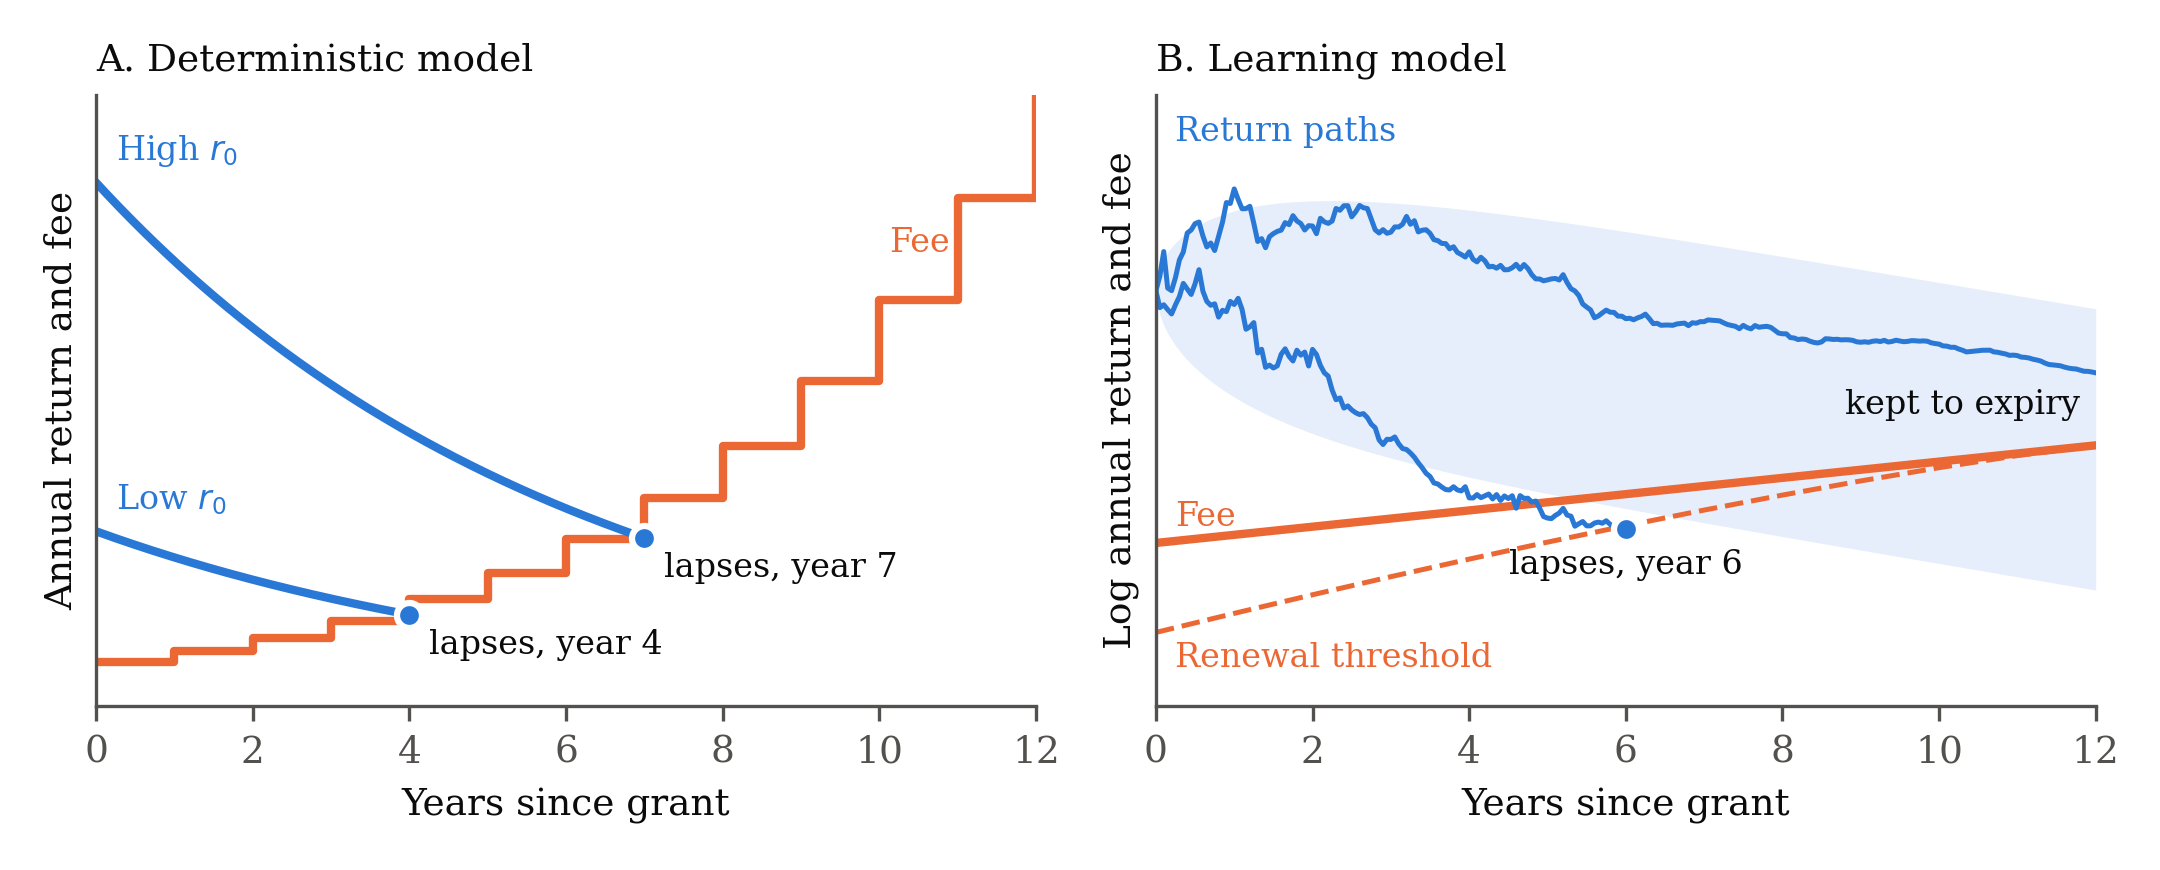
\includegraphics[width=\textwidth]{figures/fig8_models.png}
\caption{The two renewal models}\label{fig:models}
\figurenotes{Illustrative numbers, not estimates. A: a patent earns $r_0 d^t$ a year and is renewed while that
covers the fee, so the year it lapses reveals its initial return $r_0$, and the ages at which patents lapse trace out
the distribution of $r_0$. B: log returns follow a random walk with drift $\ln d$ whose shocks shrink as the owner
learns what the patent is worth (shaded: 90\% range of returns). The owner renews while the return is above a
threshold that lies below the fee by the option value of later renewals; that value vanishes at expiry.}
\end{figure}

\paragraph{Fees.} Fee schedules by year of life and period come from official sources for each office (laws,
decrees, fee regulations and office notices), with the basis of each fee: per year from filing (China, Germany, the
United Kingdom), per year from registration with a per-claim component (Korea, Japan, with ten claims assumed), three maintenance payments at 3.5, 7.5 and 11.5 years after grant (United States, with small-entity fees for firms
with fewer than 100 families and universities), per year from filing from year 3 (Russia, where foreign owners paid
a separate non-resident schedule until August 2012, in US dollars before 2009, converted at the year's exchange
rate), per year from filing from year 2 (France) or year 1 (Czech Republic, where years 1--5 were prepaid at grant
before July 2002), or per year from the grant announcement (Taiwan, whose 2002 schedule is assumed for 2000--2001). Fees are converted to 2024 PPP dollars with the consumer price index
of the year paid (for Taiwan, the DGBAS index and the IMF implied PPP rate); fees due after 2024 are held at 2024
prices. Russian lapse records end in 2022, so Russian patents are censored from mid-2022.

\paragraph{Fee discounts.} For the fee-discount estimates in Sections~\ref{sec:values} and~\ref{sec:stake}, eligible owners are domestic firms with 1--99
families and domestic universities. In China they pay 40\% of the fee in fee-years 1--3 from the grant year (to
February 2001), 30\% in fee-years 1--3 (to August 2016), 15\% in fee-years 1--6 (to July 2018) and 15\% in fee-years
1--10 (from August 2018). In Korea, registration fees for years 1--3 fall outside the model; owners pay 70\% of the
fee in years 4--6 from March 2014 and 50\% in years 4 and later from April 2018 (the extension of the 30\% discount to
years 7--9 in July 2016 is not modelled).

\paragraph{Models and decay rates.} The comparisons between owners do not depend on the model or on $d$. The ratio
of small domestic to small foreign firms' median value at equal citations is, in the deterministic model with
$d = 0.80$, 0.85 and 0.90, 2.28, 2.04 and 1.87 in China, 3.06, 2.70 and 2.45 in Korea, 1.40, 1.35 and 1.31 in the
United States, 1.69, 1.59 and 1.49 in Germany, 1.30, 1.26 and 1.23 in the United Kingdom and 5.32, 4.36 and 3.62 in
Japan; in the learning model ($d = 0.85$) it is 2.02, 2.28, 1.54, 1.53, 1.02 and 4.49. For universities the ratio
is 0.38--0.46 in China in the deterministic model and 0.27 in the learning model, against 1.02--1.07 in the United
States and 0.90--1.48 in Germany.

\begin{table}[ht]
\centering
\begin{threeparttable}
\caption{Learning model: rate of decline and fit}\label{tab:learning}
\small
% Generated by em-patent-value code/38_paper_exhibits.py (learning_model_*.csv, step 20); do not edit by hand
\begin{tabular}{lcccccccccc}
\toprule
 & CN & KR & RU & CZ & BR & US & JP & DE & GB & FR \\
\midrule
Free estimate of $d$ & 0.46 & 0.64 & 0.83 & 0.70 & 0.71 & 0.50 & 0.74 & 0.85 & 0.83 & 0.83 \\
$\sigma_0$ at $d = 0.85$ & 1.13 & 1.33 & 7.39 & 1.91 & 0.27 & 2.65 & 3.02 & 1.53 & 1.87 & 1.74 \\
Shock $s$ & 1.03 & 0.62 & 1.38 & 1.17 & 0.61 & 0.34 & 1.04 & 1.02 & 1.02 & 1.16 \\
Learning $\varphi$ & 0.94 & 0.99 & 0.94 & 0.74 & 0.82 & 0.99 & 0.99 & 0.86 & 0.83 & 0.89 \\
Fit error (pp) & 3.9 & 4.2 & 7.2 & 2.7 & 3.3 & 1.7 & 3.2 & 2.2 & 2.2 & 2.4 \\
\bottomrule
\end{tabular}
\begin{tablenotes}\footnotesize
\item \emph{Notes:} Learning model of \PaperRef{Appendix~A}{Appendix~\ref{app:models}}, estimated office by office on up to 60{,}000 patents per owner group (domestic or foreign $\times$ firm size by corporate group or university). Free estimate of $d$: the decay factor estimated with the other parameters; it is identified only where fees rise steeply every year (Germany, the United Kingdom, France) and is fixed at 0.85 in every office for the other rows. Fit error: root mean squared difference between predicted and observed shares alive 4, 8 and 12 years after grant, by owner group, weighted by patents.
\end{tablenotes}
\end{threeparttable}
\end{table}


\begin{table}[ht]
\centering
\begin{threeparttable}
\caption{Patent-level values, domestic relative to foreign owners, by office (\%)}\label{tab:patentvalues}
\small
% Generated by em-patent-value code/38_paper_exhibits.py (_tmp_values_by_office.csv); do not edit by hand
\begin{tabular}{lccccc}
\toprule
 & All owners & Small firms & Mid-sized firms & Large firms & Universities \\
 & & (1--9) & (10--99) & (100+) & \\
\midrule
\multicolumn{6}{l}{\emph{A. Emerging-market offices}} \\
China          & $33^{***}$ & $29^{***}$ & $72^{***}$ & $52^{**}$ & $-59^{***}$ \\
               & (12) & (4) & (11) & (26) & (3) \\
Korea          & $30^{***}$ & $65^{***}$ & $146^{***}$ & $16$ & $60^{**}$ \\
               & (12) & (11) & (19) & (12) & (30) \\
Russia         & $-74$ & $-3$ & $5$ & $403$ & -- \\
               & (19994989) & (61) & (84) & (825) &  \\
Czech Rep.     & $-3$ & $9$ & $-12$ & -- & -- \\
               & (16) & (22) & (20) &  &  \\
Brazil         & $7$ & $7$ & $-15$ & $23$ & $13$ \\
               & (8) & (7) & (9) & (16) & (15) \\
\addlinespace
\multicolumn{6}{l}{\emph{B. Advanced-economy offices}} \\
United States  & $41^{***}$ & $28^{***}$ & $55^{***}$ & $49^{***}$ & $14$ \\
               & (7) & (3) & (5) & (18) & (23) \\
Japan          & $144^{***}$ & $226^{***}$ & $335^{***}$ & $107^{***}$ & $516^{***}$ \\
               & (24) & (27) & (38) & (25) & (317) \\
Germany        & $0$ & $31^{***}$ & $-7$ & $-1$ & $-17$ \\
               & (7) & (8) & (7) & (9) & (27) \\
United Kingdom & $9$ & $8$ & $15$ & $12$ & $-44^{***}$ \\
               & (8) & (7) & (10) & (20) & (8) \\
France         & $-4$ & $0$ & $6$ & $-6$ & $-38^{*}$ \\
               & (9) & (8) & (11) & (12) & (17) \\
\bottomrule
\end{tabular}
\begin{tablenotes}\footnotesize
\item \emph{Notes:} Posterior median value at grant of each patent from the learning model with a common prior ($d=0.85$; 2024 PPP dollars), regressed on domestic owner with fee-path $\times$ citation-band and field effects, one regression per office and owner group (all owners: with owner-group effects); firm size by corporate group. Entries are the percentage difference in value, $100(e^{b}-1)$, with delta-method standard errors clustered by owner in parentheses; stars test $b$ on the log scale. Russian values are not identified (\PaperRef{Section~5}{Section~\ref{sec:values}}) and are shown for completeness. --: fewer than 100 domestic patents. $^{*}$~$p<0.1$, $^{**}$~$p<0.05$, $^{***}$~$p<0.01$.
\end{tablenotes}
\end{threeparttable}
\end{table}


\clearpage
\newpage 

\section{Returns at stake in the learning model}\label{app:leverslearning}

Table~\ref{tab:levers-learning} repeats Table~\ref{tab:levers} with the learning model ($d=0.85$). Each patent's
returns follow the model's random walk, and owners renew while the expected returns of keeping the patent, including
the option of later renewals, exceed the fee; a lever therefore also changes the value of that option. Markets for
technology are calibrated to the same arm's-length survival targets as in Table~\ref{tab:levers}. Because owners already keep
low-value patents for their option value, survival responds weakly to returns, and the factors are 1.30 for small
firms, 1.52 for mid-sized firms and 9.6 for universities, against 1.22, 1.40 and 3.5 in the deterministic model. The
resulting levels are several times those of Table~\ref{tab:levers} and rest on parameters that are not identified, notably the
decay rate; they are shown only to compare the levers. Fee relief is still worth about a million dollars a cohort,
so the ranking of the levers is unchanged.

\begin{table}[ht]
\centering
\begin{threeparttable}
\caption{Returns at stake per filing-year cohort, learning model (millions of 2024 PPP dollars)}\label{tab:levers-learning}
\small
% Generated by em-patent-value code/38_paper_exhibits.py (policy_levers_learning.csv, step 26b); do not edit by hand
\begin{tabular}{lccccc}
\toprule
 & \multicolumn{3}{c}{Fee relief} & Markets for technology & University patenting \\
\cmidrule(lr){2-4}\cmidrule(lr){5-5}\cmidrule(lr){6-6}
 & China & Korea & Brazil & China & China \\
\midrule
Small firms (1--9)          & 0.11 & 0.34 & 0.03 & 797 &  \\
Mid-sized firms (10--99)    & 0.04 & 0.31 & 0.02 & 1{,}194 &  \\
Large firms (100+)          & n.e. & n.e. & n.e. & 0.00 &  \\
Universities                & 0.40 & 0.26 & 0.02 & 4{,}352 & 1{,}009--1{,}460 \\
\bottomrule
\end{tabular}
\begin{tablenotes}\footnotesize
\item \emph{Notes:} As \PaperRef{Table~3}{Table~\ref{tab:levers}}, with the learning model ($d = 0.85$) on 3{,}000 patents per owner group drawn from the estimation cells; owners renew while the expected value of keeping the patent, including the option of later renewals, exceeds the fee, so each lever also changes that option. Markets for technology are calibrated to the same arm's-length survival targets as in \PaperRef{Table~3}{Table~\ref{tab:levers}}, which in this model require far larger changes in returns; the levels are not identified and are shown only to compare the levers. n.e.: not eligible.
\end{tablenotes}
\end{threeparttable}
\end{table}

